\documentclass{article}

\usepackage[UTF8]{ctex}
\usepackage{amsmath}
\usepackage{amsthm} %添加 定理 环境
\usepackage{amssymb}
\usepackage{graphicx} % 添加图片 
\usepackage{layout} % 排版版式大小更改
\usepackage{flushend, cuted} % 双栏模式实现
\usepackage{ulem} %加下划线宏包 命令 :\uline
\usepackage{fontawesome} %特殊符号超级大全
\usepackage{pifont} %带圈数字实现 ,命令:\ding{172} \ding{211}
\usepackage{fancyhdr} %页眉页脚编辑

%======================
%    解析  定理环境 定义 
%======================
\theoremstyle{plain}
\newtheorem{aly}{解析}

%======================
%    版式大小设定
%======================
\addtolength{\hoffset}{-1.5cm}
\addtolength{\voffset}{-2cm}
\addtolength{\textwidth}{2.5cm}
\addtolength{\textheight}{4cm}

%======================
%    页眉页脚设定
%======================
\pagestyle{fancy}
\fancyfoot[r]{\copyright Edited by Shine.Y}

\begin{document}

\centerline{\Large{函数值域怎么玩儿}}
\centerline{更多资讯参见 《高考调研》 32页——33页《专题研究  函数的值域》}
\vspace{10pt}

函数\textbf{值域的概念}:函数 的\emph{函数值}$y$的所有取值组成的集合就是函数的值域.

\section{求一般函数的值域}

\subsection{观察法}
\textbf{直接观察函数解析式就能得答案}

\textbf{例1.} $(1) y=x^2, y=|x|, y=\sqrt{x}$的值域都是 \uline{$[0,+\infty)$}.

\begin{aly}
  不管$x$取什么值,$x^2, |x|, \sqrt{x}$一定都大于等于$0$.
\end{aly}

$(2) y=\left\{ \begin{array}{ll}
                 2 & (x>0), \\
                 0  & (x=0), \\
                 -2 & (x<0)
               \end{array} \right.$, 的值域为 \uline{\{-2,0,2\}}.
\begin{aly}
  这个分段函数里面只出现了$2,0,-2$这三个值,一眼就能看答案。如果不能肯定,画个图出来也行。
    \begin{figure}[h]
     \centering
     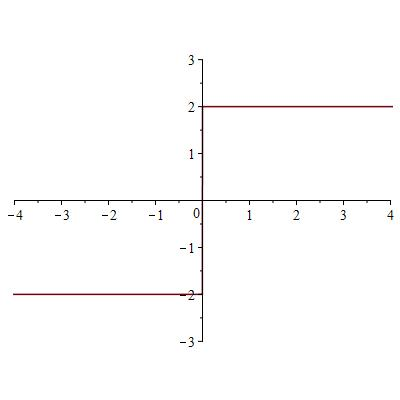
\includegraphics[width=3.5cm]{1-2.jpg}
    \end{figure}
\end{aly}

$(3) y=\left\{ \begin{array}{ll}
                 1 & (x\textrm{为有理数}), \\
                 -1 & (x\textrm{为无理数})
               \end{array} \right.$的值域为\uline{\{-1,1\}}.
\vspace{15pt}

\textbf{思考题1}

$(1) y=|x-1|$的值域为$\uline{[0,+\infty)}$;

$(2) y=(x-1)^2+2$的值域为$\uline{[2,+\infty)}$;

$(3) y=\frac{1}{x-2}+1$的值域为$\uline{(-\infty,1)\cup(1,+\infty)}$.

\begin{aly}
  此题相当于将函数$y=\frac{1}{x}$的图象向右平移$2$个单位,再向上平移$1$个单位.
\begin{figure}[h]
  \centering
  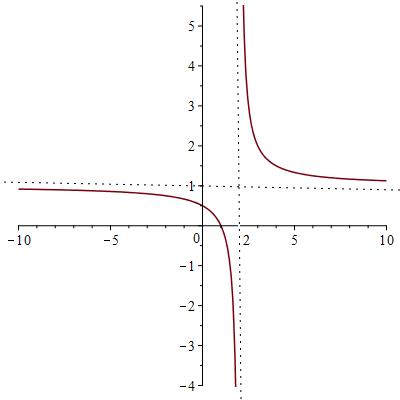
\includegraphics[width=3.5cm]{1-1-3.jpg}\label{1-1-3}
\end{figure}
\end{aly}


\subsection{配方法}
\textbf{当所求函数为二次函数类(即形如$F(x)=af^2(x)+bf(x)+c$的函数)的值域时,常用配方法}

\textbf{例2.} 求下列函数的值域.

$(1) y=x^2+4x-2, x\in \mathbf{R}$; \hspace{25pt} 答案:$[-6,+\infty)$
\begin{aly}
  $y=x^2+4x-2$这个式子可以配成\emph{顶点式}$y=(x+2)^2-6$, 那么它的图象也就出来了:
\begin{figure}[h]
  \centering
  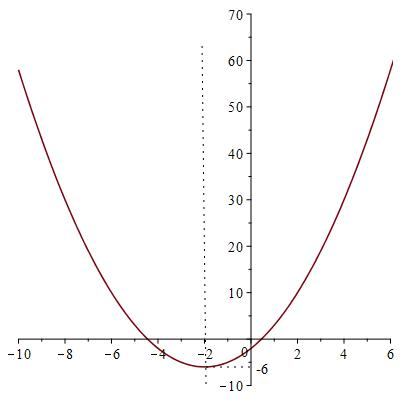
\includegraphics[width=4.5cm]{2-1.jpg}\label{2-1}
\end{figure}

看图一分析,马上得到,当$x\in \mathbf{R}$时,函数最小值为$-6$, 没有最大值,所以值域为$[-6,+\infty)$.
\end{aly}

$(2) y=x^2+4x-2, x\in [-5,0)$; \hspace{25pt} 答案:$[-6,3]$
\begin{figure}[h]
  \centering
  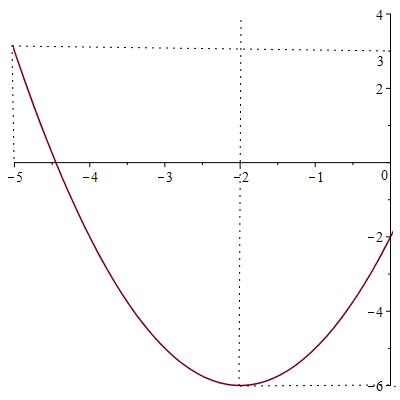
\includegraphics[width=4cm]{2-2.jpg}
  \label{2-2}
\end{figure}

$(3) y=x^2+4x-2, x\in [-6,-3]$; \hspace{25pt} 答案:$[-5,10]$

$(4) y=x^2+4x-2, x\in [0,2]$. \hspace{25pt} 答案:$[-2,10]$
\vspace{15pt}

\textbf{思考题2}

$(1) $函数$y=x^4+x^2+1$的值域是$\uline{[1,+\infty)}$; $y=x^4-x^2+1$的值域是$\uline{[ \frac{3}{4},+\infty)}$.

\begin{aly}
  \begin{description}
     \item[对于函数$\mathbf{y=x^4+x^2+1}$] 这个式子可以配成\emph{顶点式} $y=(x^2+\frac{1}{2})^2+\frac{3}{4}$(这里自变量$x$的取值范围默认是全体实数范围), 但是要\textbf{注意}这里$x^2$始终大于等于 $0$, 也就是说 $x^2+\frac{1}{2}$ 的最小值为 $\frac{1}{2}$, 那么 $(x^2+\frac{1}{2})^2$ 的最小值为 $\frac{1} {4}$, 则 $(x^2+\frac{1}{2})^2+\frac{3}{4}$ 的最小值为$1$, 没有最大值,那么这个函数的值域就是 $[1,+\infty)$.
     \item[对于函数$\mathbf{y=x^4-x^2+1}$] 这个式子和上面的式子的不同之处在于上面的式子是 $\mathbf{+x^2}$, 下面的式子是 $\mathbf{-x^2}$. 下面这个式子可以配成\emph{顶点式} $y=(x^2-\frac{1}{2})^2+\frac{3}{4}$(这里自变量$x$的取值范围默认是全体实数范围), 虽然这里 $x^2$ 依然大于等于 $0$, 但是当 $x^2=\frac{1}{2}$ 时,$(x^2-\frac{1}{2})^2$ 就可以等于 $0$ 了,$(x^2-\frac{1}{2})^2$ 的取值范围就是 $[0,+\infty)$, 那么整体的 $ (x^2-\frac{1}{2})^2+\frac{3}{4}$ 的取值范围就是 $[\frac{3}{4},+\infty)$, 这也就是函数的值域.
   \end{description}
\end{aly}

(2) 求下列函数的值域.

\ding{172} $y=\sqrt{-x^2+4x-1}$; \hspace{25pt} 答案:$[0,\sqrt{3}]$

\begin{aly}
  只要解决了根号下面的那一整个式子的取值范围,相应的函数值 $y$ 的取值范围也确定了.

  而 $-x^2+4x-1$ 的顶点式表示就是 $-(x-2)^2+3$, 图象开口向下,其最大值就是 $3$, 又因为 $-x^2+4x-1$ 在根号下面,所以它一定大于等于 $0$. 规范的解答书写过程如下:\\
  解:$\because y=\sqrt{-x^2+4x-1}$\\
  $\therefore y=\sqrt{-(x-2)^2+3}$\\
  又$\because 0 \leqslant -(x-2)^2+3 \leqslant 3$\\
  $\therefore 0 \leqslant \sqrt{-(x-2)^2+3} \leqslant \sqrt{3}$\\
  $\therefore$ 该函数的值域为 $[0, \sqrt{3}]$.
\end{aly}

\ding{173} $y=2-\sqrt{4x-x^2} (0 \leqslant x \leqslant 4)$; \hspace{25pt} 答案:$[0,2]$

\begin{aly}
  同样的,先把 $4x-x^2$ 的取值范围找出来,因为这是一个二次函数式,可以直接画出它在$0 \leqslant x \leqslant 4$ 这段范围对应的图象,接着找出这个整体的取值范围,然后一步步地变到 $2-\sqrt{4x-x^2}$ 的形式去. 规范的解答书写过程如下:\\
  解:$\because 0 \leqslant x \leqslant 4$\\
  $\therefore 0 \leqslant 4x-x^2 \leqslant 4$\\
  $\therefore 0 \leqslant \sqrt{4x-x^2} \leqslant 2$\\
  $\therefore -2 \leqslant -\sqrt{4x-x^2} \leqslant 0$\\
  $\therefore 0 \leqslant 2-\sqrt{4x-x^2} \leqslant 2$\\
  $\therefore$ 该函数的值域为$[0,2]$.
\end{aly}


\subsection{换元法}
\textbf{就一句话,用 $t$ 去替换掉 复杂带根号 的那一坨}

\textbf{例3.} 求函数 $y=x-\sqrt{1-2x}$ 的值域. \hspace{25pt} 答案:$(-\infty, \frac{1}{2}]$
\begin{aly}
  这个式子和上面思考题2 (2) \ding{173} $y=2-\sqrt{4x-x^2}$ 那个式子的一个很大的区别点在于,其中一个式子\textbf{根号}里面外面都有 $x$, 而另一个式子只有\textbf{根号}里面才有 $x$, 所以两种题目的解法是不一样的,大家不要弄混淆了. 规范的解答书写过程如下:\\
  解:令 $t=\sqrt{1-2x} (t \geqslant 0)$, \\
  则 $t^2=1-2x$\\
  $2x=1-t^2$\\
  $x=\frac{1-t^2}{2}$\\
  $\therefore y=\frac{1-t^2}{2}-t$\\
  $y=\frac{1}{2}-\frac{1}{2}t^2-t$\\
  $y=-\frac{1}{2}t^2-t+\frac{1}{2}$\\
  $\because t \geqslant 0$\\
  $\therefore -\frac{1}{2}t^2-t+\frac{1}{2} \leqslant \frac{1}{2}$\\
  $\therefore y \leqslant \frac{1}{2}$\\
  $\therefore$ 该函数的值域为 $(-\infty, \frac{1}{2}]$
\end{aly}

\textbf{思考题3} 求下列函数的值域.

(1) $y=2x-3+\sqrt{4x-13}$; \hspace{25pt} 答案:$[\frac{7}{2}, +\infty)$

(2) $y=2x-1-\sqrt{13-4x}$; \hspace{25pt} 答案:$(-\infty, \frac{11}{2}]$

(3) $y=(x-2)^2+2|x-2|-1$; \hspace{25pt} 答案:$[-1, +\infty)$

\begin{aly}
  这道题里面,$(x-2)^2$ 就相当于是 $(|x-2|)^2$, 那么这个式子就可以改写为 $y=(|x-2|)^2+2|x-2|-1$. 用 $t$ 去替换 $|x-2|$, 并且 $t \geqslant 0$, 就可以得到 $y=t^2+2t-1$, 把这个二次函数式解出来就行.  规范的解答书写过程如下:\\
  解:$\because y=(x-2)^2+2|x-2|-1$\\
  $\therefore y=(|x-2|)^2+2|x-2|-1$\\
  令 $t=|x-2| (t \geqslant 0)$, 则\\
  $y=t^2+2t-1$\\
  $y=(t+1)^2-2$\\
  $\because$ 当 $t \geqslant 0$ 时,\\
  $(t+1)^2-2 \geqslant -2$\\
  $\therefore y \geqslant -2$\\
  $\therefore$ 该函数的值域为 $[-2, +\infty)$.
\end{aly}



\subsection{分离常数法}
\textbf{将式子改写为一个经过上下左右平移的\emph{反比例函数式}}

\textbf{例4.} 求函数 $y=\frac{x+1}{x+2}$ 的值域. \hspace{25pt} 答案:$(-\infty, 1) \cup (1, +\infty)$

\begin{aly}
  规范的解答书写过程如下:\\
  解:$\because y=\frac{x+1}{x+2}$\\
  $\therefore y=\frac{x+2-1}{x+2}$\\
  $y=1-\frac{1}{x+2}$\\
  $y=-\frac{1}{x+2}+1$\\
  $\therefore$ 该函数的值域为 $(-\infty, 1) \cup (1, +\infty)$.
\end{aly}

\textbf{思考题4} 求函数 $y=\frac{5-x}{2x+5}$ 的值域. \hspace{25pt} 答案:$(-\infty, -\frac{1}{2}) \cup (-\frac{1}{2}, +\infty)$

\begin{aly}
  将这个函数式变形为 \[y=\frac{-\frac{1}{2}(2x+5)+\frac{15}{2}}{2x+5}\]就能得出答案了.
\end{aly}


\subsection{判别式法}
\textbf{把函数式转化为关于x的二次方程,通过已知方程有实根,即判定 $\Delta \geqslant 0$, 从而求得原函数的值域. }

\textbf{例5} 求函数 $y=\frac{x^2-2x+3}{x^2+2x-3}$ 的值域. \hspace{25pt} 答案:$(-\infty, -1) \cup (\frac{1}{2}, +\infty)$

\begin{aly}
  将这个函数式改写为关于 $x$ 的二次方程,具体的解答过程如下: \\
  解:$\because y=\frac{x^2-2x+3}{x^2+2x-3}$
  (其中 $x^2+2x-3 \neq 0$, 也即 $x \neq -1$ 和 $3$)\\
  $\therefore (x^2+2x-3)y=x^2-2x+3$\\
  $\therefore yx^2+2yx-3y=x^2-2x+3$\\
  $\therefore (y-1)x^2+2(y+1)x-3(y+1)=0$\\
  \ding{172} 当 $y=1$ 时,$x=\frac{3}{2}$ 在定义域内\\
  \ding{173} 当 $y \neq 1$ 时,$\Delta \geqslant 0$, \\
  即 $(2(y+1))^2-4(y-1)(-3(y+1)) \geqslant 0$\\
  $\therefore y \geqslant \frac{1}{2}$ 或 $y \leqslant -1$\\
  $\therefore$ 该函数的值域为 $(-\infty, -1) \cup (\frac{1}{2}, +\infty)$.
\end{aly}

\textbf{思考题5} 求下列函数的值域.

(1) $y=\frac{2x^2-6x+5}{2x^2-6x+6}$; \hspace{25pt} 答案:$[\frac{1}{3}, 1)$

(2) $y=\frac{2x^2+2x+5}{x^2+x+1}$; \hspace{25pt} 答案:$(2, 6]$


\subsection{单调性法}
\textbf{若函数在某个区间内具有单调性,则可借助单调性求值域. 常用于对勾函数求值域. }

\textbf{例6} 求函数 $y=x+\frac{2}{x} (0 < x < 1)$ 的值域. \hspace{25pt} 答案:$(3, +\infty)$

\begin{aly}
  这就是一个对勾函数,我们可以直接画出它的图象来找出值域,也可以通过严谨的推导过程来获得答案,规范的解答书写过程如下:\\
  解:任取$x_1,x_2 \in (0,1)$, 设 $x_1 < x_2$\\
  $f(x_1)-f(x_2)=x_1+\frac{2}{x_1}-(x_2+\frac{2}{x_2})$ \\
       $=x_1-x_2+\frac{2}{x_1}-\frac{2}{x_2}$\\
       $=(x_1-x_2)+2(\frac{1}{x_1}-\frac{1}{x_2})$\\
       $=(x_1-x_2)+2(\frac{x_2-x_1}{x_1x_2})$\\
       $=(x_1-x_2)(1-\frac{2}{x_1x_2})$\\
       $=\frac{(x_1-x_2)(x_1x_2-2)}{x_1x_2}$\\
  $\because x_1 <x_2 \quad \therefore x_1-x_2 < 0$\\
  又 $\because 0 < x < 1 \quad \therefore x_1x_2 > 0, x_1x_2-2 < 0$\\
  $\therefore f(x_1)-f(x_2) > 0$\\
  $\therefore f(x_1) > f(x_2)$\\
  $\therefore f(x)$ 在 $(0,1)$ 上为减函数\\
  当 $x=1$ 时,$f(1)=3$\\
  $\therefore$ 该函数的值域为 $(3, +\infty)$.
\end{aly}

\textbf{思考题6} 求函数 $y=x+\frac{1}{x}(x\neq 0)$ 的值域. \hspace{25pt} 答案:$(-\infty, -2]\cup [2, +\infty)$


\subsection{数形结合法}
\textbf{常见用于形如$f(x)=|g(x)|+|h(x)|$的函数,关键就在于去掉“$|\quad|$”符号,$x$ 应当如何取值. }

\textbf{例7} 求函数 $y=|x+3|+|x-5|$ 的值域. \hspace{25pt} 答案:$[8, +\infty)$

\begin{aly}
  想要去掉式子中的 “$|\quad|$”符号,就得先搞清楚,当 $x$ 取何值时,去掉绝对值符号要变号,之后就以这些刚好要变号的值作为分界点,对不同 $x$ 取值情况进行讨论,就能写出一个分段函数了,写出来之后,把分段函数的图象画出来就成. 具体解答过程如下:\\
  解:$\because y=|x+3|+|x-5|$\\
  $\therefore y=\left\{
  \begin{array}{ll}
     -2x+2 & (x < -3) \\
     8 & (-3 \leqslant x < 5) \\
     2x-2 & (x \geqslant 5)
  \end{array}\right.$
\begin{figure}[h]
  \centering
  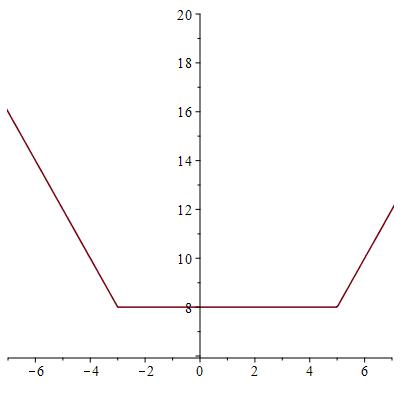
\includegraphics[width=4.5cm]{7-1.jpg}
\end{figure}

  $\therefore$ 该函数的值域为 $[8,+\infty)$.
\end{aly}

\textbf{思考题7} 求函数 $y=|x-2|-|x+1|$ 的值域. \hspace{25pt} 答案:$[-3,3]$
\begin{aly}
  该函数式改写为分段函数为:
  $y=\left\{
    \begin{array}{ll}
    3 & (x < -1) \\
    -2x+1 & (-1 \leqslant x < 2) \\
    -3 & (x \geqslant 2)
  \end{array}\right.$  \\之后画出分段函数图象来就能判断出函数值域. 当然你也可以牢记下面关于\textbf{求分段函数的值域}的那一句话.
\end{aly}


\section{求分段函数的值域}
\textbf{分段函数的值域为每一区间函数的值域的并集}

\section{求复合函数的值域}
\textbf{复合函数的值域即为外层函数的值域}

\end{document} 